\section{Базовый эксперимент}
Для проведения эксперимента, из данных электрокортикограммы были выделены частоты сигналов. Выходные данные~--- трехмерные координаты движения руки обезьяны. Полученные данные были разделены на обучающую и контрульную выборки в отношении два к одному. На полученной выборке был обучен PLS с различным количеством компонент (от 2 до 100). Для оценки качества предсказания использовались метрики mean squared error, mean absolute error и r2 score. Результаты эксперимента представлены на рис.~\ref{fig:baseAlgo}.
\begin{figure}
  \begin{center}
    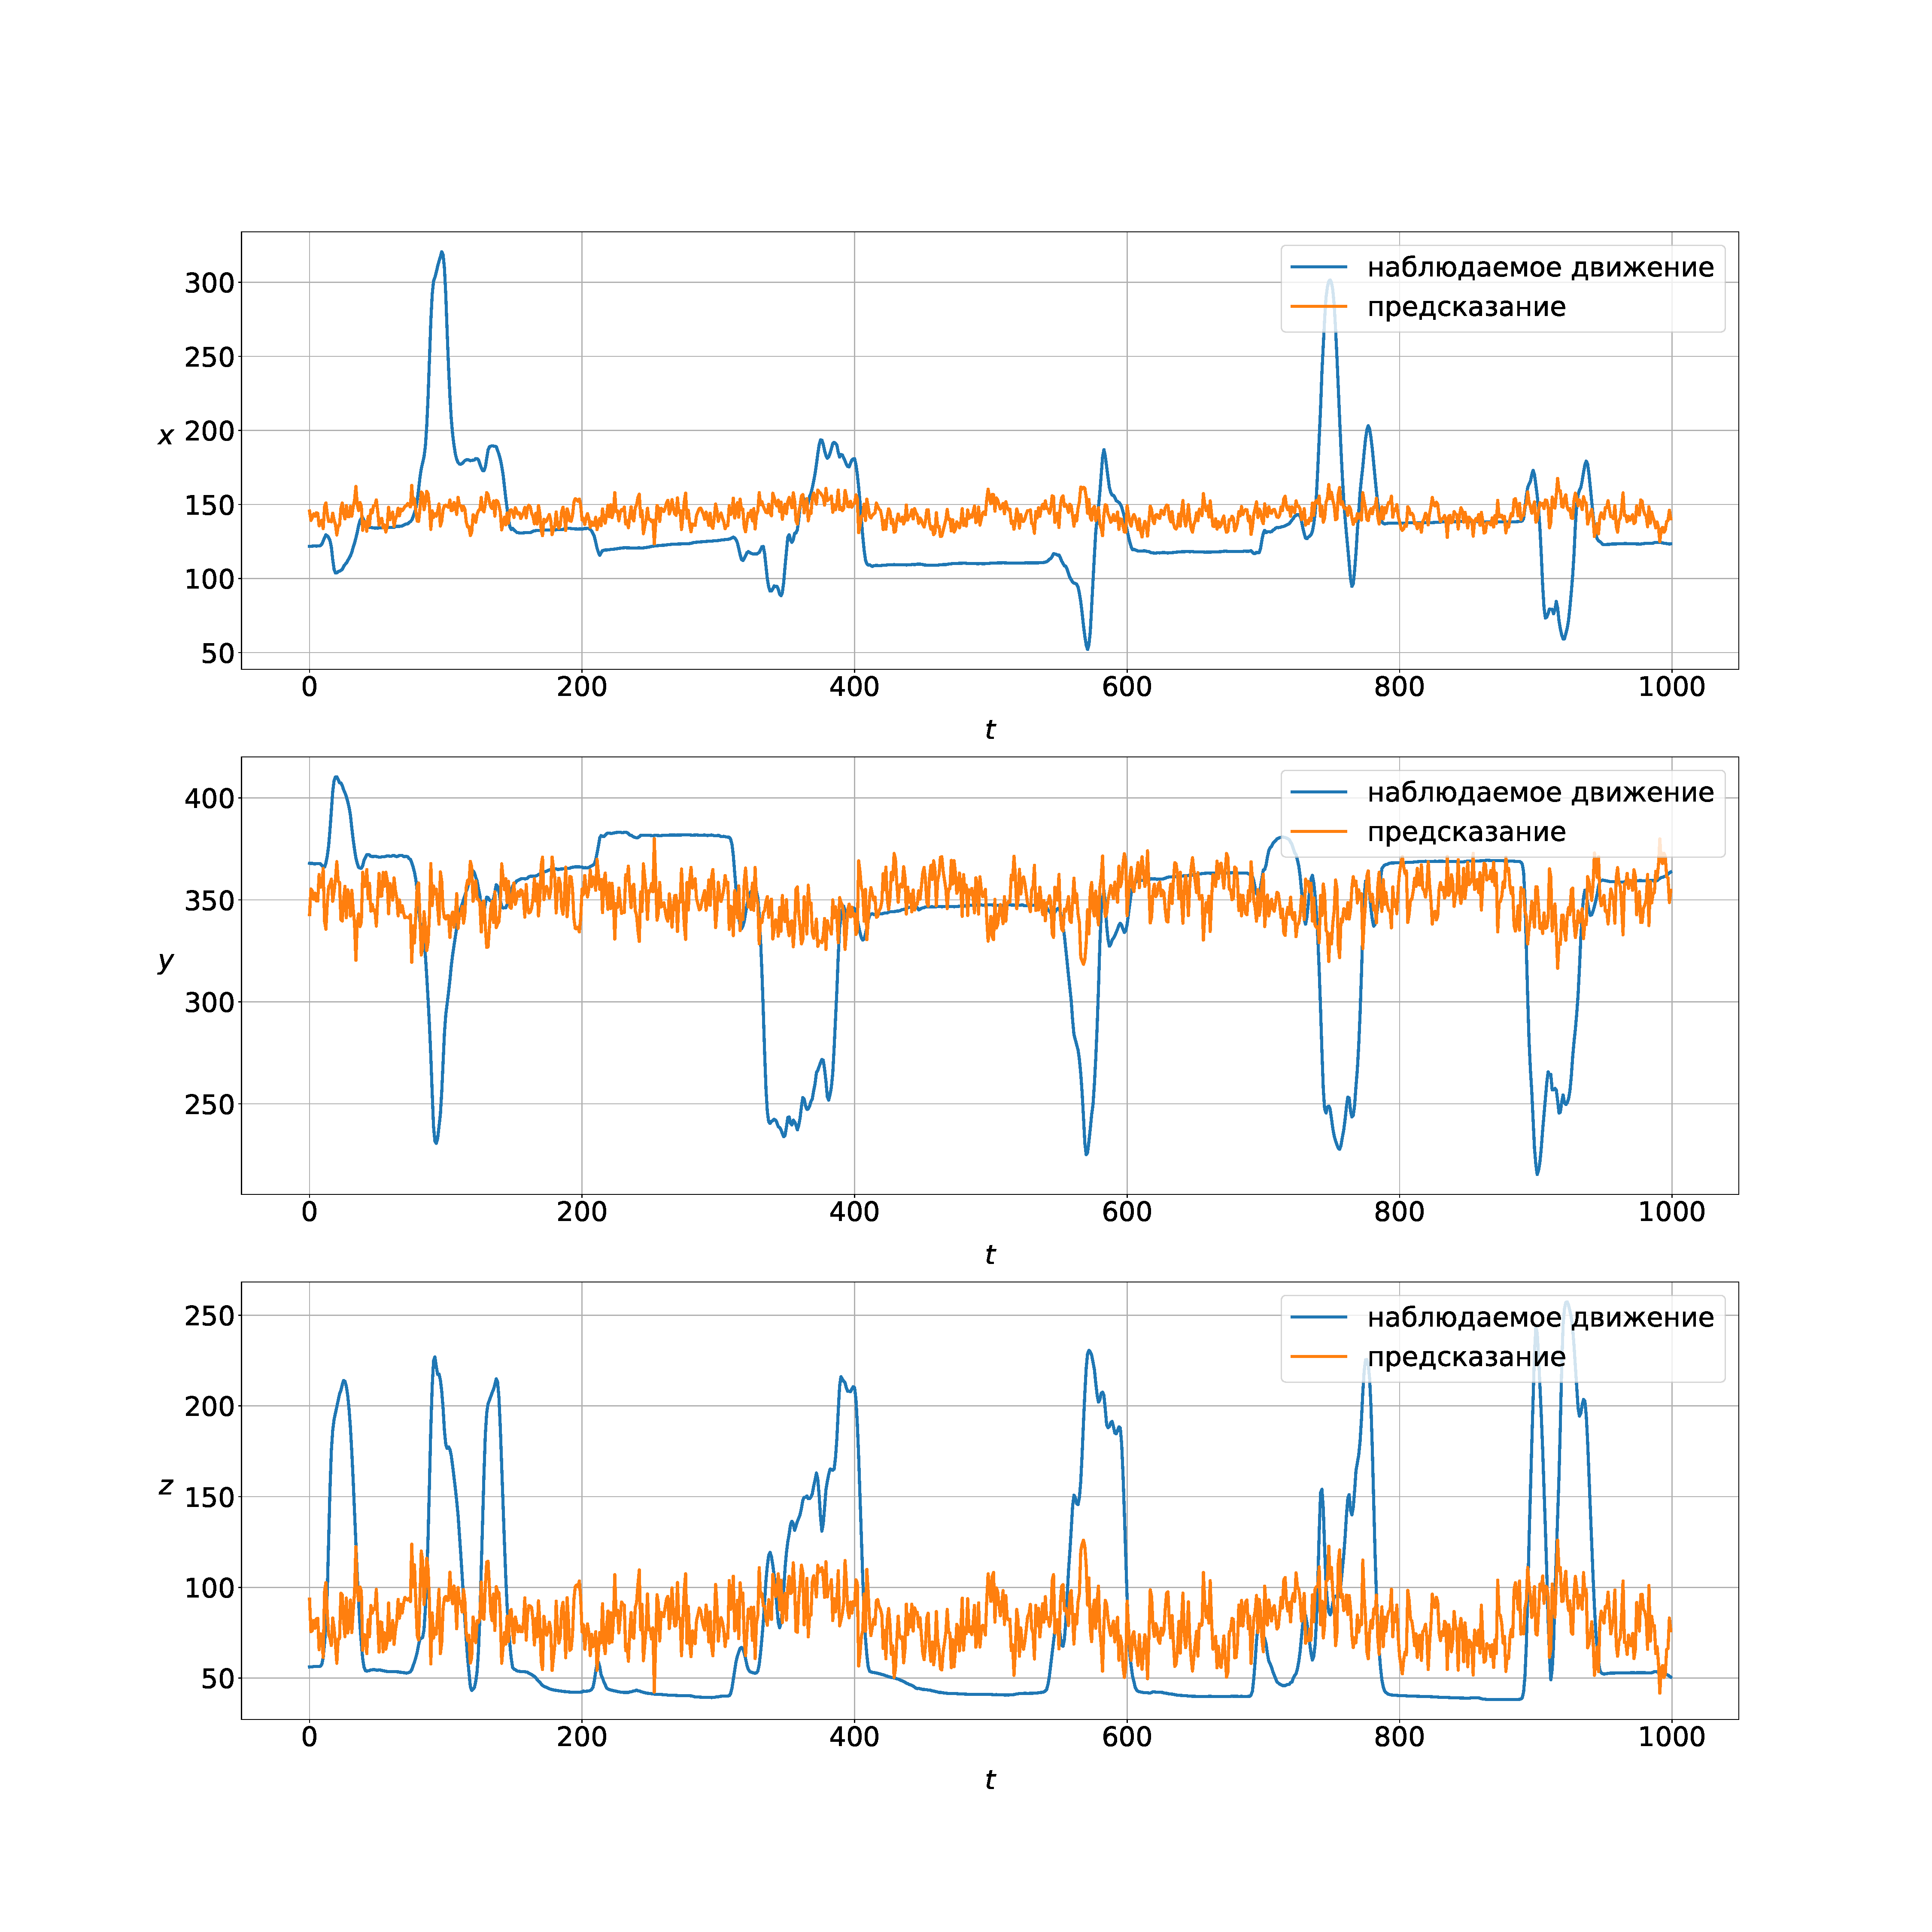
\includegraphics[width=\textwidth]{base_algo.pdf}
    \caption{Результаты предсказания движения с помощью двухкомпонентного PLS}
    \label{fig:baseAlgo}
  \end{center}
\end{figure}
На графике представлена зависимость координаты конечности от времени. Как видно из рисунка, базовый алгоритм довольно плохо справляется с поставленной задачей. Общий профиль пиков соблюдается, однако PLS очень грубо оценивает острые пики. Также предсказание испытывает флуктуации, когда конечность почти не движется. В результате погрешность предсказания высока. Эксперимент показал значения метрик $mae = 30.17, mse = 1843.91, r2 = 0.01$. Для борьбы с погрешностями предлагается снизить размерность входного сигнала.
